\documentclass[lang=cn,newtx,10pt,scheme=chinese]{elegantbook}

\title{数学分析学习笔记}
\subtitle{复习整理笔记}

\author{阮炜挺}
\institute{宁波大学数学与统计学院}
\date{}

\extrainfo{Given yourself an epsilon of room!}

\setcounter{tocdepth}{3}

\cover{cover.jpg}

% 本文档命令
\usepackage{array}
\newcommand{\ccr}[1]{\makecell{{\color{#1}\rule{1cm}{1cm}}}}

% 修改标题页的橙色带
\definecolor{customcolor}{RGB}{32,178,170}
\colorlet{coverlinecolor}{customcolor}
\usepackage{cprotect}

\addbibresource[location=local]{reference.bib} % 参考文献,不要删除
\everymath{\displaystyle} % 使所有公式默认使用行间公式
\usepackage{extarrows}

\begin{document}

\maketitle
\frontmatter

\tableofcontents

\mainmatter

\chapter{含参变量积分}

\section{基本定理}

\begin{theorem}[连续性]
设 $f(x,t)$ 在 $[a,b] \times [c,d]$ 上连续, 则 $\varphi(t) = \int_{a}^{b} f(x,t) dx$ 在 $[c,d]$ 上连续, 即
$$ \lim\limits_{t \to t_0} \int_{a}^{b} f(x,t) dx = \int_{a}^{b} f(x, t_0) dx = \int_{a}^{b} \lim\limits_{t \to t_0} f(x,t) dx, \quad \forall t_0 \in [c,d]. $$
\end{theorem}

\begin{theorem}[交换积分次序]
设 $f(x,t)$ 在 $[a,b] \times [c,d]$ 上连续, 则
$$ \int_{c}^{d} dt \int_{a}^{b} f(x,t) dx = \int_{a}^{b} dx \int_{c}^{d} f(x,t) dt. $$
\end{theorem}

\begin{theorem}[可微性]
设 $f(x,t), f_t(x,t)$ 在 $[a,b] \times [c,d]$ 上连续, 则 $\varphi(t) = \int_{a}^{b} f(x,t) dx$ 在 $[c,d]$ 上可导, 且
$$ \varphi'(t) = \int_{a}^{b} f_t(x,t) dx. $$
\end{theorem}

\begin{theorem}[一般情形的连续性与可微性]
设 $f(x,t)$ 在 $[a,b] \times [c,d]$ 上连续, 函数 $\alpha(t), \beta(t)$ 在 $[c,d]$ 上连续, 且 $a \le \alpha(t), \beta(t) \le b, \forall t \in [a,b]$, 则 $\varphi(t) = \int_{\alpha(t)}^{\beta(t)} f(x,t) dx$ 在 $[c,d]$ 上连续. 进一步, 若 $f_t(x,t)$ 在 $[a,b] \times [c,d]$ 上连续, $\alpha(t), \beta(t)$ 在 $[c,d]$ 上可导, 则 $\varphi(t)$ 也在 $[c,d]$ 上可导, 且
$$ \varphi'(t) = f[\beta(t),t]\beta'(t) - f[\alpha(t),t]\alpha'(t) + \int_{\alpha(t)}^{\beta(t)} f_t(x,t) dx. $$
\end{theorem}

\section{含参变量正常积分}

\subsection{简单例题}
\begin{example}
设 $f(x,y) = \operatorname{sgn}(x-y)$, 证明: 含参量积分 $F(y) = \int_{0}^{1} f(x,y) \,dx$ 在 $(-\infty, +\infty)$ 上连续.
\end{example}
\begin{solution}
对$y$的范围进行讨论有$F(y) = \begin{cases} 1, & y < 0, \\ 1-2y, & 0 \le y \le 1, \\ -1, & y > 1. \end{cases} $ $\blacksquare$
\end{solution} 

\begin{example}
设 $x>0$, 且 $f(x) = \int_{x}^{x^2} \frac{\sin ux}{u} \,du$, 求 $f'(x)$.
\end{example}
\begin{solution}
\begin{align*}
f'(x) &= 2x \cdot \frac{\sin x^3}{x^2} - \frac{\sin x^2}{x} + \int_{x}^{x^2} \cos ux \,du = \frac{2\sin x^3 - \sin x^2}{x} + \frac{\sin ux}{x} \bigg|_{x}^{x^2} = \frac{3\sin x^3 - 2\sin x^2}{x}. \blacksquare
\end{align*}

\end{solution}

\begin{example}[$\bigstar$]
设 $f(x)$ 在 $[0,1]$ 上连续, 讨论函数 $F(t) = \int_0^1 \frac{t}{x^2+t^2}f(x)dx$ 的连续性.
\end{example}

\begin{solution}
令 $g(x,t) = \frac{t}{x^2+t^2}f(x)$, 那么 $F(t) = \int_0^1 g(x,t) dx$. 注意到 $F(t)$ 是奇函数.
$\forall t_0 \in (0, +\infty)$, $g(x,t)$ 在 $[0,1] \times [\frac{t_0}{2}, 2t_0]$ 中连续, 那么 $F(t)$ 在 $[\frac{t_0}{2}, 2t_0]$ 连续.
从而 $F(t)$ 在 $t_0$ 点连续, 从而 $F(t)$ 在 $(0, +\infty)$ 连续. 同理 $F(t)$ 在 $(-\infty, 0)$ 也连续, 故 $F(t)$ 在 $(-\infty, 0) \cup (0, +\infty)$ 连续.

接下来讨论 $t=0$ 处. 首先有 $F(0)=0$. 再考虑
$$ \lim\limits_{t \to 0^+} F(t) = \boxed{\lim\limits_{t \to 0^+} \int_0^1 \frac{t}{x^2+t^2}f(x)dx }$$
我们将积分拆分为两部分:
$$ \int_0^1 \frac{t}{x^2+t^2}f(x)dx = \int_0^{t^{\frac{1}{4}}} \frac{t}{x^2+t^2}f(x)dx + \int_{t^{\frac{1}{4}}}^1 \frac{t}{x^2+t^2}f(x)dx = I_1 + I_2 $$
\begin{enumerate}
    \item 对于 $I_1 = \int_0^{t^{\frac{1}{4}}} \frac{t}{x^2+t^2}f(x)dx$, 由积分中值定理, 存在 $\xi \in (0, t^{\frac{1}{4}})$, 使得
    $$ I_1 = f(\xi) \int_0^{t^{\frac{1}{4}}} \frac{t}{x^2+t^2}dx = f(\xi)\left[\arctan \frac{x}{t}\right]_0^{t^{\frac{1}{4}}} = f(\xi) \arctan\frac{t^{\frac{1}{4}}}{t} = f(\xi) \arctan\frac{1}{t^{\frac{3}{4}}} $$
    那么当 $t \to 0^+$ 时, $\xi \to 0$, $\arctan\frac{1}{t^{\frac{3}{4}}} \to \frac{\pi}{2}$.
    从而
    $$ \lim\limits_{t \to 0^+} I_1 = \lim\limits_{t \to 0^+} f(\xi) \arctan\frac{1}{t^{\frac{3}{4}}} = f(0) \cdot \frac{\pi}{2} $$
    \item 对于 $I_2 = \int_{t^{\frac{1}{4}}}^1 \frac{t}{x^2+t^2}f(x)dx$, 由于 $f$ 在 $[0,1]$ 上连续, 故有界, 不妨设 $|f(x)| \le M$. 那么
    $$ |I_2| \le M \int_{t^{\frac{1}{4}}}^1 \frac{t}{x^2+t^2}dx = M \left(\arctan \frac{1}{t} - \arctan \frac{t^{\frac{1}{4}}}{t}\right) = M\left(\arctan\frac{1}{t} - \arctan\frac{1}{t^{\frac{3}{4}}}\right) $$
    由于当 $t \to 0^+$ 时, $\arctan\frac{1}{t} \to \frac{\pi}{2}$ 且 $\arctan\frac{1}{t^{\frac{3}{4}}} \to \frac{\pi}{2}$, 故 $\lim\limits_{t \to 0^+} M\left(\arctan\frac{1}{t} - \arctan\frac{1}{t^{\frac{3}{4}}}\right) = 0$.
    所以 $\lim\limits_{t \to 0^+} I_2 = 0$.
\end{enumerate}
由 1 和 2 可知 $\lim\limits_{t \to 0^+} F(t) = \frac{\pi}{2}f(0) + 0 = \frac{\pi}{2}f(0)$.
因为 $F(t)$ 是奇函数, 同理可得 $\lim\limits_{t \to 0^-} F(t) = -\lim\limits_{t \to 0^+} F(-t) = -F(0^+) = -\frac{\pi}{2}f(0)$.
$F(t)$ 在 $t=0$ 处连续的充要条件是左右极限存在且等于 $F(0)=0$.
$$ \lim\limits_{t \to 0^+} F(t) = \lim\limits_{t \to 0^-} F(t) = F(0) \implies \frac{\pi}{2}f(0) = -\frac{\pi}{2}f(0) = 0 $$
这等价于 $f(0)=0$.
所以, 当 $f(0)=0$ 时, $F(t)$ 在 $t=0$ 处连续. 当 $f(0) \neq 0$ 时, $F(t)$ 在 $t=0$ 处不连续.$\hfill \blacksquare$
\end{solution}

\begin{example}
证明函数 $J(x) = \frac{1}{\pi}\int_{0}^{\pi} \cos(t - x \sin t) \,dt$ 满足
$$ x^2 J''(x) + x J'(x) + (x^2 - 1)J(x) = 0. $$
\end{example}
\begin{note}
    操作过程中用分部积分把积分中的三角函数统一名称即可,需要注意的是分部积分过程中要看清楚是对哪个变量进行求导.此题也说明有时候通过简单的四则运算并不能消去所有项,这题最后剩下了一个积分为零的项.
\end{note}

\begin{solution}
首先注意到
\begin{align*}
J'(x) &= \frac{1}{\pi} \int_{0}^{\pi} \sin(t - x\sin t)\sin t \,dt = -\frac{1}{\pi} \int_{0}^{\pi} \sin(t - x\sin t) \,d(\cos t) \\
&= -\frac{1}{\pi}\sin(t-x\sin t)\cos t \bigg|_{0}^{\pi} + \frac{1}{\pi} \int_{0}^{\pi} \cos(t - x\sin t)(1 - x\cos t)\cos t \,dt  \text{\color{red}(注意分部积分的变量是t)}\\
&= \frac{1}{\pi} \int_{0}^{\pi} \cos(t-x\sin t)\cos t \,dt - \frac{x}{\pi}\int_{0}^{\pi} \cos(t-x\sin t)\cos^2 t \,dt.
\end{align*}
另外, 还有
\begin{align*}
J''(x) &= \frac{1}{\pi} \int_{0}^{\pi} \cos(t-x\sin t)(-\sin^2 t) \,dt \\
&= \frac{1}{\pi} \int_{0}^{\pi} \cos(t-x\sin t)\cos^2 t \,dt - \frac{1}{\pi}\int_{0}^{\pi} \cos(t-x\sin t) \,dt.
\end{align*}
由此可知
\begin{align*}
x^2 J''(x) + x J'(x) + (x^2-1)J(x) = -\frac{1}{\pi}\big[\sin(t-x\sin t)\big]_{0}^{\pi} = 0.\blacksquare
\end{align*}


\end{solution}

\begin{example}
设 $f(x)$ 在 $a$ 的某邻域内具有连续的 $n+1$ 阶导函数, 求 $\lim\limits_{x \to a} \frac{d^n}{dx^n} \left[ \frac{f(x) - f(a)}{x-a} \right]$.
\end{example}

\begin{solution}
注意到 $x \neq a$ 时, 有
$$ \boxed{\frac{f(x)-f(a)}{x-a} = \int_{0}^{1} f'(a+t(x-a)) \,dt}. $$
因此
$$ \frac{d^n}{dx^n} \left[ \frac{f(x)-f(a)}{x-a} \right] = \int_{0}^{1} f^{(n+1)}(a+t(x-a))\cdot t^n \,dt. $$
再结合 $f^{(n+1)}(x)$ 的\underline{连续性}, 有
$$ \lim\limits_{x \to a} \frac{d^n}{dx^n} \left[ \frac{f(x)-f(a)}{x-a} \right] = \int_{0}^{1} \lim\limits_{x \to a} \left\{ f^{(n+1)}[a+t(x-a)] \cdot t^n \right\} dt = f^{(n+1)}(a) \int_{0}^{1} t^n \,dt = \frac{f^{(n+1)}(a)}{n+1}. $$
\hfill $\blacksquare$
\end{solution}

\begin{example}
设 $F(t) = \int_{0}^{t} dx \int_{x^2}^{t^2} f(x,y) \,dy$, 其中 $f(x,y)$ 为连续函数, 求 $F'(t)$.
\end{example}

\begin{solution}
即定理1.4的应用.
记 $g(x,t) = \int_{x^2}^{t^2} f(x,y) \,dy$, 则 $F(t) = \int_{0}^{t} g(x,t) \,dx$,又因为$g_t(x,t) = f(x,t^2)\cdot 2t + \int_{x^2}^{t^2} f_t(x,y)dy = 2tf(x,t^2)$,
从而有$F'(t) = g(t,t)+\int_{0}^{t}g_t(x,t)dx = \int_{0}^{t}2tf(x,t^2)dx$ $blacksquare$.
\end{solution}
\begin{note}
    累次含参变量积分的处理方法,通过设 $g(x,t)$ 为积分的被积函数, 来化为一般形式的含参变量积分.
\end{note}

\begin{example}
设 $F(t) = \int_0^a dx \int_0^a f(x+y+t) dy$, 其中 $f$ 为连续函数. 证明
$$F''(t) = f(t+2a) - 2f(t+a) + f(t).$$
\end{example}

\begin{proof}
由于 $f$ 只是连续函数, 故不能直接对积分号下的 $f$ 求二阶导数.
令 $g(x,t) = \int_0^a f(x+y+t) dy$, 从而 $F(t) = \int_0^a g(x,t) dx$.
不妨设 $f$ 的原函数为 $H$, $H$ 的原函数为 $G$. (即 $H'=f, G'=H, G''=f$)
那么
$$ g(x,t) = \int_0^a f(x+y+t) dy = \big[ H(x+y+t) \big]_{y=0}^{y=a} = H(x+t+a) - H(x+t). $$
而
\begin{align*}
F(t) &= \int_0^a g(x,t) dx = \int_0^a [H(x+t+a) - H(x+t)] dx \\
&= \big[ G(x+t+a) \big]_{x=0}^{x=a} - \big[ G(x+t) \big]_{x=0}^{x=a} \\
&= [G(a+t+a) - G(0+t+a)] - [G(a+t) - G(0+t)] \\
&= G(t+2a) - G(t+a) - G(t+a) + G(t) \\
&= G(t+2a) - 2G(t+a) + G(t).
\end{align*}
那么
$$ F''(t) = \frac{d^2}{dt^2} [G(t+2a) - 2G(t+a) + G(t)] = G''(t+2a) - 2G''(t+a) + G''(t). $$
因为 $G''=f$, 所以
$$ F''(t) = f(t+2a) - 2f(t+a) + f(t) \blacksquare$$
\end{proof}

\begin{example}[$\bigstar$]
计算累次积分 $\int_0^1 dx \int_0^1 \frac{x^2 - y^2}{(x^2 + y^2)^2} dy$ 与  $\int_0^1 dy \int_0^1 \frac{x^2 - y^2}{(x^2 + y^2)^2} dx$.
\end{example}

\begin{solution}
    令$$P(x,y) = \frac{x}{(x^2 + y^2)}, Q(x,y) = \frac{y}{(x^2 + y^2)}$$ 注意到$$P_x(x,y) = \frac{y^2 - x^2}{(x^2 + y^2)^2}, Q_y(x,y) = \frac{x^2 - y^2}{(x^2 + y^2)^2}$$
    且有$-P_x(x,y) = Q_y(x,y)$

    那么
    $$
    \int_0^1 dx \int_0^1 \frac{x^2 - y^2}{(x^2 + y^2)^2} dy = \int_0^1 dx \int_0^1 Q_y(x,y) dy = \int_0^1 Q(x,y) \bigg|_{y=0}^{y=1} dx = \int_0^1 \frac{1}{1+x^2} dx = \frac{\pi}{4}.
    $$
    同理
    $$
    \int_0^1 dy \int_0^1 \frac{x^2 - y^2}{(x^2 + y^2)^2} dx = \int_0^1 dy \int_0^1 -P_x(x,y) dx = \int_0^1 -P(x,y) \bigg|_{x=0}^{x=1} dy = -\int_0^1 \frac{1}{1+y^2} dy = -\frac{\pi}{4}.
    $$
    $\hfill \blacksquare$
\end{solution}

\subsection{含参变量积分的计算}
\begin{proposition}
当 $|a|<1$ 时, 有
\begin{equation*}
\int \frac{dx}{1+a\cos x} = \frac{2}{\sqrt{1-a^2}} \arctan\left(\sqrt{\frac{1-a}{1+a}}\tan\frac{x}{2}\right) + C. 
\end{equation*}

特别地, 有
\begin{equation*}
\int_{0}^{\pi} \frac{dx}{1+a\cos x} = \frac{\pi}{\sqrt{1-a^2}}, \quad |a|<1. 
\end{equation*}
类似的还有
$$
\int_{0}^{\pi} \frac{1}{a + \cos x} dx = \frac{\pi}{\sqrt{a^2 - 1}}, \quad a > 1.
$$

$$
\int_{0}^{\pi} \frac{1}{a + \cos x} dx =  - \frac{\pi}{\sqrt{a^2 - 1}}, \quad a < 1.
$$
\end{proposition}
\begin{remark}
    此命题用万能公式即可.
\end{remark}

如果直接求$\varphi(t) = \int_{a}^{b}f(x,t) \mathrm d x$有困难,那么通常采用以下两种方法:
\textcolor{blue}{\begin{enumerate}
    \item \textbf{积分号下积分}:把$f(x,t)$表示为积分形式,再用积分号下求积分的方法,此时通常要交换积分次序,所以要先判断函数的连续性.
    \item \textbf{积分号下微分}:先求$\varphi'(t)$,即先求$\int_{a}^{b}f_t(x,t) \mathrm d x$,然后再对$t$积分求出$\varphi(t)$,所以要先判断$f(x,t)$和$f_t(x,t)$的连续性.
\end{enumerate}}

\subsubsection{积分号下积分}

\begin{example}
计算 $\int_0^1 \frac{x^b - x^a}{\ln x} dx$, 其中 $0 < a < b$.
\end{example}

\begin{solution}
注意到 $$\frac{x^b - x^a}{\ln x} = \left[ \frac{x^y}{\ln x} \right]_{y=a}^{y=b} = \int_a^b x^y dy$$
那么
\begin{align*}
\int_0^1 \frac{x^b - x^a}{\ln x} dx &= \int_0^1 dx \int_a^b x^y dy \quad (\text{由于 } x^y \text{ 在 } [0,1] \times [a,b] \text{ 上连续, 故可交换积分次序}) \\
&= \int_a^b dy \int_0^1 x^y dx = \int_a^b \left[ \frac{x^{y+1}}{y+1} \right]_{x=0}^{x=1} dy = \int_a^b \frac{1}{y+1} dy \\
&= \big[ \ln(y+1) \big]_{y=a}^{y=b} = \ln(b+1) - \ln(a+1) = \ln\frac{b+1}{a+1}. 
\end{align*}
$ \hfill \blacksquare$
\end{solution}

\begin{example}
计算 $\int_0^1 \sin\left(\ln\frac{1}{x}\right)\frac{x^b - x^a}{\ln x}dx$ 与 $\int_0^1 \cos\left(\ln\frac{1}{x}\right)\frac{x^b - x^a}{\ln x}dx$, 其中 $0 < a < b$.
\end{example}

\begin{solution}
注意到 $\frac{x^b - x^a}{\ln x} = \int_a^b x^y dy$, 那么$\int_0^1 \sin\left(\ln\frac{1}{x}\right)\frac{x^b - x^a}{\ln x}dx = \int_0^1dx\int_a^b x^y\sin(\ln\frac 1 x)dy$,

令$f(x,y) = x^y\sin(\ln\frac 1 x)$, 且有$\lim_{x \to 0^+} f(x,y) = 0,\forall y \in [a,b]$,那么可以令
$$F(y) = \begin {cases}
 x^y\sin(\ln\frac 1 x),&0< x \leq 1 \\
    0,  &x = 0.
\end{cases}$$
从而$F(x,y)$在$[0,1] \times [a,b]$ 上连续, 故积分可以交换次序, 从而有
$$
\int_0^1 \sin\left(\ln\frac{1}{x}\right)\frac{x^b - x^a}{\ln x}dx =\int_0^1 dx \int_a^b f(x,y) dy =\int_{0}^{1} dx \int_{a}^{b} F(x,y) dy = \int_a^b dy \int_0^1 F(x,y) dx = \int_a^b dy \int_0^1 x^y \sin(\ln\frac{1}{x}) dx
$$
令$u = \ln \frac{1}{x}$,那么上式可化为
$$\int_a^b dy \int_0^{+\infty} e^{-u} e^{-yu} \sin u \,du = \int_a^b dy \int_0^{+\infty} e^{-(y+1)u} \sin u \,du$$
\begin{figure}[h]
	\centering 
	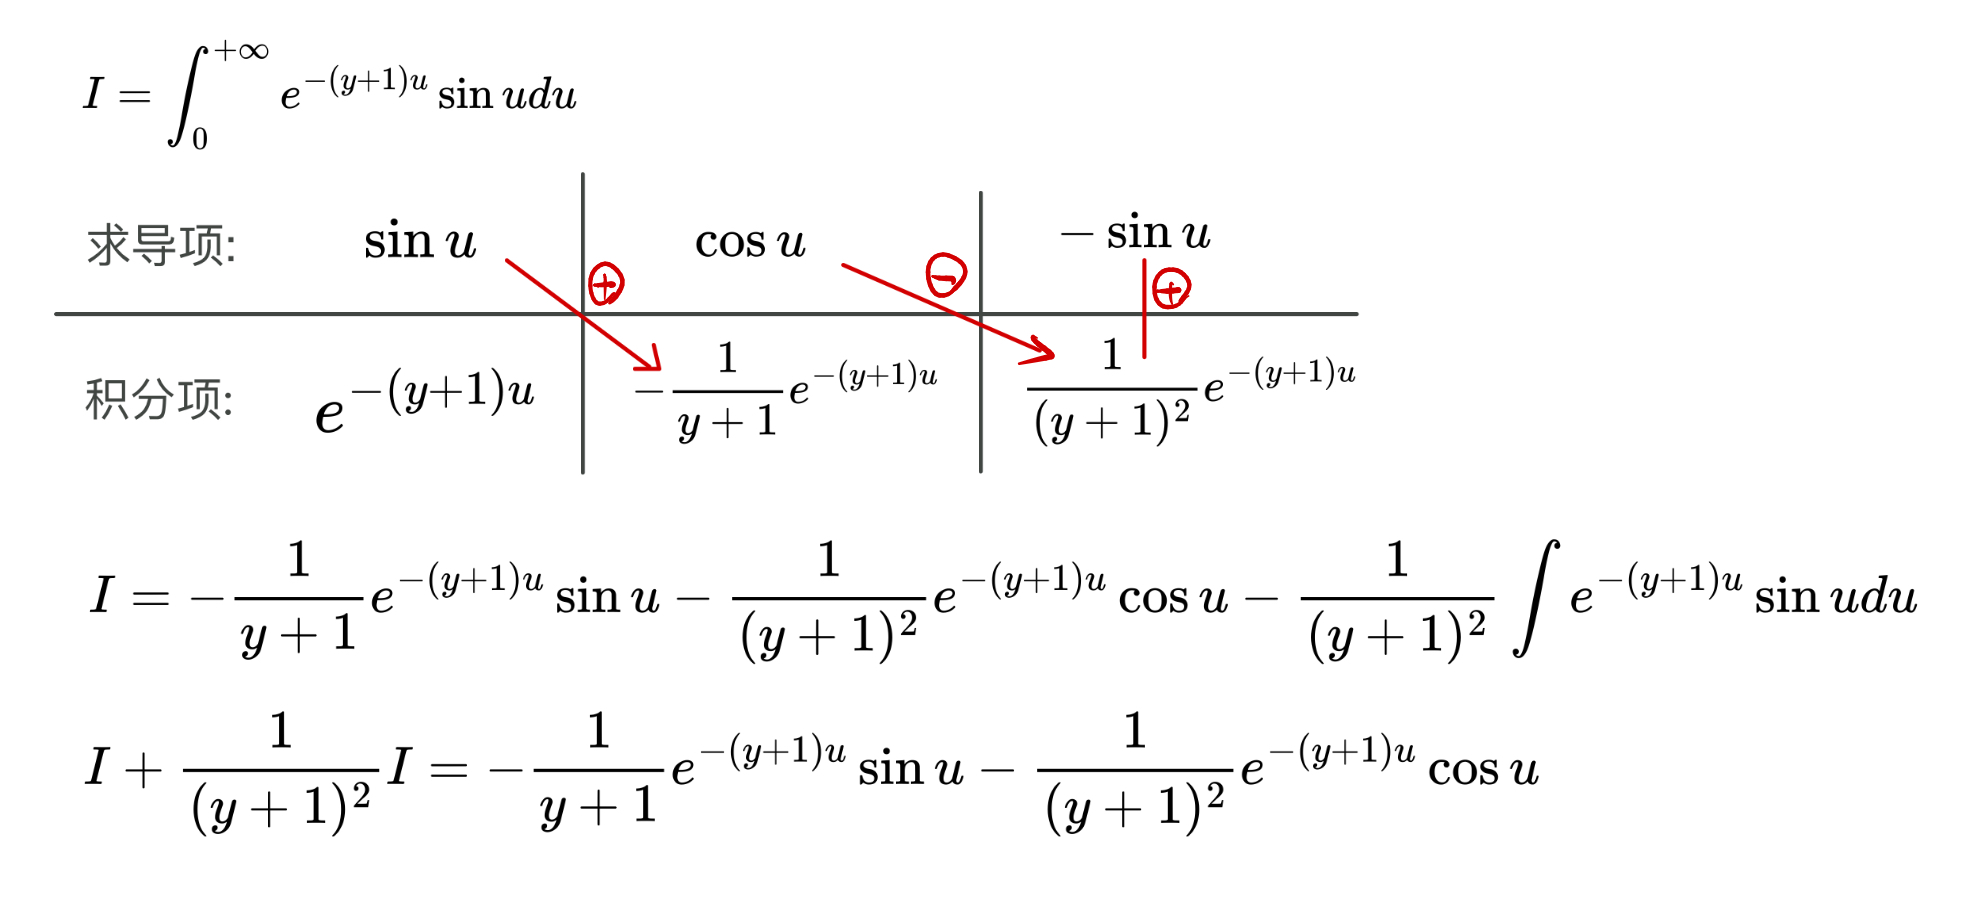
\includegraphics[width=0.9\textwidth]{表格法1.jpg} 
\end{figure}

右边将上下限代入即得
$$\int_0^1 \sin\left(\ln\frac{1}{x}\right)\frac{x^b - x^a}{\ln x}dx = \int_a^b \frac{1}{(y+1)^2 + 1} dy = \arctan(b+1) - \arctan(a+1).$$

同理可得
\begin{align*}
    \int_0^1 \cos\left(\ln\frac{1}{x}\right)\frac{x^b - x^a}{\ln x}dx &= \int_a^b dy \int_0^{+\infty} e^{-(y+1)u} \cos u \,du = \int_{a}^{b} \frac{y+1}{(y+1)^2 +1}dy \\
&= \frac{1}{2} \ln\left((y+1)^2 + 1\right) \bigg|_{y=a}^{y=b} =  \frac 1 2 \ln\frac{(b+1)^2 + 1}{(a+1)^2 + 1}. \blacksquare
\end{align*}
\end{solution}

\begin{example}
计算 $F(\alpha) = \int_{0}^{\frac{\pi}{2}} \ln\frac{1+\alpha\cos x}{1-\alpha\cos x} \cdot \frac{1}{\cos x}dx$, 其中 $\alpha \in (-1,1)$.
\end{example}

\begin{solution}
$$ F(\alpha) = \int_0^{\frac{\pi}{2}} \frac{\ln(1+\alpha\cos x) - \ln(1-\alpha\cos x)}{\cos x} dx =\int_0^{\frac{\pi}{2}} dx \int_{-\alpha}^{\alpha} \frac{1}{1+y\cos x} dy $$
此时, 令 $f(x,y) = \frac{1}{1+y\cos x}$, 该函数在区域 $[0, \frac{\pi}{2}] \times [-\alpha, \alpha]$ 上连续. 故积分次序可交换.
\begin{note}
    寻找函数的过程:
    
    积分里是$\frac{\ln(1+\alpha\cos x) - \ln(1-\alpha\cos x)}{\cos x}=\frac{\ln(1+y\cos x)}{\cos x}\bigg|_{y=-\alpha}^{y=\alpha}$,那么对$\frac{\ln(1+y\cos x)}{\cos x}$关于$y$求导即可得积分中的被积函数,在此例中求导后得到的就是$\frac{1}{1+y\cos x}$
\end{note}

\begin{align*}
\int_0^{\frac{\pi}{2}} dx \int_{-\alpha}^\alpha \frac{1}{1+y\cos x} dy &
= \int_{-\alpha}^\alpha dy \int_0^{\frac{\pi}{2}} \frac{1}{1+y\cos x} dx \\
& = \color{blue}{\boxed{\int_{-\alpha}^0 dy \int_0^{\frac{\pi}{2}} \frac{dx}{1+y\cos x} + \int_0^\alpha dy \int_0^{\frac{\pi}{2}} \frac{dx}{1+y\cos x}}} \color{red}{\text{(利用对称性)}}\\
& = \int_0^\alpha dy \int_0^{\frac{\pi}{2}} \frac{dx}{1-y\cos x} + \int_0^\alpha dy \int_0^{\frac{\pi}{2}} \frac{dx}{1+y\cos x} \\
& = \int_0^\alpha dy \int_0^{\frac{\pi}{2}} \frac{2dx}{1-y^2\cos^2 x} = \int_0^\alpha dy \int_0^{\frac{\pi}{2}} \frac{2\sec^2 x dx}{\tan^2 x + (1-y^2)} \\
& = \int_0^\alpha dy \int_0^{\frac{\pi}{2}} \frac{2}{\tan^2 x + (1-y^2)} d(\tan x) = \int_0^\alpha \frac{2}{\sqrt{1-y^2}} \arctan \frac{\tan x}{\sqrt{1-y^2}} \bigg|_0^{\frac{\pi}{2}} dy \\
& = \pi \int_0^\alpha \frac{dy}{\sqrt{1-y^2}} = \pi \arcsin \alpha, \quad \alpha \in (-1,1)
\end{align*}
$\hfill \blacksquare$
\end{solution}

\subsubsection{积分号下微分}
我们先来证明欧拉积分:
\begin{proposition}[欧拉积分]
$$I = \int_0^{\frac{\pi}{2}} \ln \cos t \, dt =I = \int_0^{\frac{\pi}{2}} \ln \sin u \, du = -\frac{\pi}{2}\ln 2$$
\end{proposition}

\begin{proof}
    考虑 $I = \int_0^{\frac{\pi}{2}} \ln \cos t \, dt$
    令 $u = \frac{\pi}{2} - t$, 则 $I = \int_0^{\frac{\pi}{2}} \ln \sin u \, du$
    将上面两式子相加有:
    $$2I = \int_0^{\frac{\pi}{2}} (\ln \cos t + \ln \sin t) \, dt = \int_0^{\frac{\pi}{2}} \ln (\frac{1}{2} \sin 2t) \, dt = -\frac{\pi}{2}\ln 2 + \int_0^{\frac{\pi}{2}} \ln (\sin 2t) \, dt$$
    令 $u = 2t$, 则积分变为 
    \begin{align*}
    \int_0^{\frac{\pi}{2}} \ln (\sin 2t) \, dt &= \frac{1}{2} \int_0^\pi \ln \sin u \, du =  \frac{1}{2} \int_0^{\frac{\pi}{2}} \ln \sin u \, du + \frac{1}{2} \int_{\frac{\pi}{2}}^{\pi} \ln \sin u \, du (\text{第二个积分中令}v = \frac{\pi}{2}- u)\\
     &=  \frac{1}{2} \int_0^{\frac{\pi}{2}} \ln \sin u \, du + \frac{1}{2} \int_{0}^{\frac{\pi}{2}} \ln \cos v \, dv =\frac{1}{2} \cdot 2I = I
    \end{align*}
    那么 $2I = -\frac{\pi}{2}\ln 2 + I \Rightarrow I = -\frac{\pi}{2}\ln 2$ $\hfill \blacksquare$
\end{proof}


\begin{example}[$\bigstar$]{\label{ex:integral-parameter_1}}
    计算$F(\theta)= \int_{0}^{\pi} \ln (1+\theta \cos x) \mathrm{d} x$,其中$\theta \in [-1,1]$.
\end{example}

\begin{solution}
令$f(x, \theta) = \ln(1+\theta \cos x)$, 其中$\theta \in [-1, 1]$. 注意到当$\theta = \pm 1$时, $f(x, \theta)$可能无界. 先对这两种情形讨论.
$1^\circ \theta = \pm 1$时
$$F(1) = \int_{0}^{\pi} \ln(1+\cos x)dx = \int_{0}^{\pi} \ln(2\cos^2\frac{x}{2})dx = \pi\ln2 + 2\int_{0}^{\pi}\ln(\cos\frac{x}{2})dx$$$$= \pi\ln2 + 4\int_{0}^{\pi}\ln(\cos\frac{x}{2})d(\frac{x}{2}) = \pi\ln2 + 4\int_{0}^{\frac{\pi}{2}}\ln\cos x dx = \pi\ln2 - 4 \times \frac{\pi}{2}\ln2$$$$= -\pi\ln2$$
同理$F(-1) = \int_{0}^{\pi} \ln(1-\cos x)dx = \pi\ln2 + 4\int_{0}^{\frac{\pi}{2}}\ln\sin x dx = -\pi\ln2$

$2^\circ$ 当$\theta \in (-1, 1)$时
$f'_{\theta}(x, \theta) = \frac{\cos x}{1+\theta \cos x}$, 那么此时$f(x, \theta), f'_{\theta}(x, \theta)$在$[0, \pi] \times (-1, 1)$均连续, 那么$F(\theta)$在$(-1, 1)$可导.
又因为
\begin{equation*}
F(-\theta) = \int_{0}^{\pi} \ln(1-\theta\cos x)dx \xlongequal{t=\pi-x} \int_{0}^{\pi} \ln(1+\theta\cos t)dt = F(\theta)
\end{equation*}

从而$F(\theta)$为偶函数, 那样就先求它在$(x, \theta) \in [0, \pi] \times [0, 1)$上的情形.
考虑
\begin{align*}
    F'(\theta) &= \int_{0}^{\pi} \frac{\cos x}{1+\theta \cos x}dx = \color{blue}{\frac{1}{\theta}\int_{0}^{\pi}\frac{1+\theta\cos x - 1}{1+\theta\cos x}dx} = \frac{1}{\theta}\int_{0}^{\pi}(1-\frac{1}{1+\theta\cos x})dx \\
               &= \frac{\pi}{\theta} - \frac{1}{\theta}\int_{0}^{\pi}\frac{1}{1+\theta\cos x}dx = \frac{\pi}{\theta} - \frac{\pi}{\theta\sqrt{1-\theta^2}}, |\theta|<1
\end{align*}


那么
\begin{align*}
    F(\theta)&=\int(\frac{\pi}{\theta}-\frac{\pi}{\theta\sqrt{1-\theta^2}})d\theta = \pi\ln\theta - \pi\int\frac{1}{\theta\sqrt{1-\theta^2}}d\theta+C =\pi \ln \theta - \color{blue}{\int\frac{\theta^{-2}\pi}{\sqrt{\theta^{-2}-1}}\mathrm{d} \theta +C}\\
             &=\pi \ln \theta + \int\frac{\pi}{\sqrt{\theta^{-2}-1}}\mathrm{d} \theta^{-1} +C = \pi \ln \theta +\pi \ln(\theta^{-1}+\sqrt{\theta^{-2}-1})+C=\pi \ln (1+ \sqrt{1-\theta^2}) +C
\end{align*}

当$\theta=0, F(0)=\lim\limits_{\theta \to 0} F(\theta) = \pi\ln2+C$, 而$F(0)=0$, 故$C=-\pi\ln2$.
那么$F(\theta)=\pi\ln\frac{1+\sqrt{1-\theta^2}}{2}$, 此时$F(\theta)$为偶函数.
那么在$(-1, 1)$上,$F(\theta)=\pi\ln\frac{1+\sqrt{1-\theta^2}}{2}$.

综上由$1^\circ, 2^\circ$得$F(\theta)=\pi\ln\frac{1+\sqrt{1-\theta^2}}{2}, \theta \in [-1, 1]$.
$\hfill \blacksquare$
\end{solution}

\begin{note}
    与本题类似的还有
        先计算含参变量积分$$I(\alpha) = \int _0^{\pi} \ln(\alpha +\cos x)dx,\alpha > 1$$
    易知$f(\alpha,x)$可导,且
    $$ I'(\alpha) = \int_{0}^{\pi} \frac{1}{\alpha + \cos x} dx \stackrel{t=\tan\frac{x}{2}}{=} \int_{0}^{+\infty} \frac{1}{\alpha + \frac{1-t^2}{1+t^2}} \cdot \frac{2 dt}{1+t^2}  = 2 \int_{0}^{+\infty} \frac{dt}{\alpha(1+t^2) + 1-t^2} = 2 \int_{0}^{+\infty} \frac{dt}{\alpha+1 + (\alpha-1)t^2} $$
    $$ = \frac{2}{\sqrt{\alpha^2-1}} \int_{0}^{+\infty} \frac{1}{1 + \left(\sqrt{\frac{\alpha-1}{\alpha+1}}t\right)^2} d\left(\sqrt{\frac{\alpha-1}{\alpha+1}}t\right)  = \frac{2}{\sqrt{\alpha^2-1}} \left( \arctan \sqrt{\frac{\alpha-1}{\alpha+1}}t \right) \Bigg|_{0}^{+\infty} = \frac{2}{\sqrt{\alpha^2-1}} \cdot \frac{\pi}{2} = \frac{\pi}{\sqrt{\alpha^2-1}} $$
    那么$I(\alpha) = \pi ln(\alpha +\sqrt{\alpha^2 -1})+C$,且$I(1)=\pi ln(1+0)+C=C$.

    而$I(1) = -\pi\ln 2$(降次加欧拉积分即可得).那么$C = I(1) = -\pi \ln 2$,则
    $$I(\alpha) = \pi ln(\alpha +\sqrt{\alpha^2 -1})+C= \pi ln(\alpha +\sqrt{\alpha^2 -1})-\pi \ln 2=\pi \ln \frac{\alpha+\sqrt{\alpha^2 -1}}{2}  $$$\hfill \blacksquare$
\end{note}

\begin{example}[$\bigstar$]
    计算$F(a) = \int_0^{\pi} \ln(a^2 -2a \cos x +1) \mathrm{d} x$.
\end{example}

\begin{solution}[解法1]


\begin{remark}
考虑$a^2-2a\cos x+1$, 视为$a$的二次函数.
有$\Delta=4\cos^2x-4 \le 0$. 则$\Delta < 0$时, $f(x,a)=\ln(a^2-2a\cos x+1)$有意义.
当$\Delta=0$, 即$\cos^2x=1$, 即$\cos x=\pm 1$时, $f(x,a)=\ln(a\mp 1)^2$可能无意义.
此时需对$a=\pm 1$进行讨论.
\end{remark}

$1^\circ$ 当$a=\pm 1$时
$F(1) = \int_{0}^{\pi}\ln(1-2\cos x+1)dx = \int_{0}^{\pi}(\ln 2+\ln(1-\cos x))dx = \pi\ln2 - \pi\ln2=0$,
同理有$F(-1) = \int_{0}^{\pi}\ln(1+2\cos x+1)dx=0$

$2^\circ$ 当$|a|<1$时. $F(-a)=F(a)$. 故先考虑$0<a<1$.
$f_a(x,a) = \frac{2a-2\cos x}{a^2-2a\cos x+1}$,由于$f(x,a)$,$f_a(x,a)$在$[0,\pi] \times (0,1)$上连续, 故可以求导.
即有$F'(a)=\int_{0}^{\pi}\frac{2a-2\cos x}{a^2-2a\cos x+1}dx$

\begin{align*}
    F'(a) &= \color{blue}{\frac{1}{a}\int_{0}^{\pi}\frac{a^2-2a\cos x+1-(1-a^2)}{a^2-2a\cos x+1}dx = \frac{1}{a}\int_{0}^{\pi}(1-\frac{1-a^2}{a^2-2a\cos x+1})dx}\\
          &= \frac{\pi}{a} - \frac{1-a^2}{a}\int_{0}^{\pi}\frac{1}{a^2+1-2a\cos x}dx = \frac{\pi}{a} - \frac{1-a^2}{a(1+a^2)}\int_{0}^{\pi}\frac{1}{1-\frac{2a}{1+a^2}\cos x}dx \\
          &= \frac{\pi}{a} - \frac{1-a^2}{a(1+a^2)}\frac{\pi}{\sqrt{1-(\frac{2a}{1+a^2})^2}} = \frac{\pi}{a} - \frac{1-a^2}{a(1+a^2)}\frac{\pi(a^2+1)}{|a^2-1|} = \frac{\pi}{a} - \frac{\pi}{a}\cdot\frac{1-a^2}{1-a^2} = 0
\end{align*}

从而$F(a)=C$. 又由$F(0)=0$, 而$\lim\limits_{a\to 0}F(a)=0$, 故$C=0$, 那么$F(a)=0$.
且$F(a)$为偶函数, 那么当$-1<a<1$时, $F(a)=0$.

$3^\circ$ 当$|a|>1$时, $|\frac{1}{a}|<1$,那么有

\begin{align*}
F(\frac{1}{a}) &= \int_{0}^{\pi}\ln\left(\frac{1}{a^2}-\frac{2\cos x}{a}+1\right)dx = \int_{0}^{\pi}\ln\frac{1-2a\cos x+a^2}{a^2}dx \\
&= \int_{0}^{\pi}\ln(1-2a\cos x+a^2)dx - 2\pi\ln|a| = F(a)-2\pi\ln|a|
\end{align*}

又由于$F(\frac{1}{a}) = 0 $,故 $F(a) = \begin{cases} 2\pi\ln|a|, & |a| \geq  1 \\ 0, & |a|<  1 \end{cases}$
$\hfill \blacksquare$
\end{solution}

\begin{solution}[解法2]
\begin{align*}
F(a) &= \int_{0}^{\pi} \ln(a^2 - 2a\cos x + 1)dx = \int_{0}^{\pi} \ln(a^2+1-2a\cos x)dx \\
&= \int_{0}^{\pi} \ln\left((a^2+1)\left(1-\frac{2a}{a^2+1}\cos x\right)\right)dx = \int_{0}^{\pi}\ln(a^2+1)dx + \int_{0}^{\pi}\ln\left(1-\frac{2a}{a^2+1}\cos x\right)dx \\
&= \pi\ln(a^2+1) + \int_{0}^{\pi}\ln\left(1-\frac{2a}{a^2+1}\cos x\right)dx, \quad \text{由于 } |\frac{2a}{a^2+1}| \le 1, \text{再利用上题结论} \\
&= \pi\ln(a^2+1) + \pi\ln\frac{1+\sqrt{1-\left(\frac{2a}{a^2+1}\right)^2}}{2} = \pi\ln\frac{a^2+1}{2} + \pi\ln\left(1+\sqrt{1-\frac{4a^2}{(a^2+1)^2}}\right) \\
&= \pi\ln\frac{a^2+1}{2} + \pi\ln\left(1+\sqrt{\frac{a^4+2a^2+1-4a^2}{(a^2+1)^2}}\right) = \pi\ln\frac{a^2+1}{2} + \pi\ln\left(1+\sqrt{\frac{(a^2-1)^2}{(a^2+1)^2}}\right) \\
&= \pi\ln\frac{a^2+1}{2} + \pi\ln\left(1+\frac{|a^2-1|}{a^2+1}\right) = \pi\ln\frac{a^2+1+|a^2-1|}{2} \\
&= \begin{cases}
2\pi\ln|a|, & |a| \ge 1 \\
0, & |a| < 1
\end{cases}
\end{align*}
$\hfill \blacksquare$
\end{solution}

\begin{solution}[解法3]
        当 $|a| < 1$ 时,注意到$I(a)=I(-a)$,则有:
    \begin{align*} 2I(a) &= \int_{0}^{\pi} \ln(1-2a\cos x + a^2)dx + \int_{0}^{\pi} \ln(1+2a\cos x + a^2)dx \\ &= \int_{0}^{\pi} \ln(1-2a^2\cos 2x + a^4)dx = \frac{1}{2} \int_{0}^{2\pi} \ln(1-2a^2\cos x + a^4)dx \\ &= \int_{0}^{\pi} \ln(1-2a^2\cos x + a^4)dx = I(a^2)\end{align*}
    从而:
    $$ I(a) = \lim\limits_{n \to \infty} \frac{I(a^{2^n})}{2^n} $$
    考虑极限
    $$ \lim\limits_{n \to \infty} I(a^{2^n}) = \lim\limits_{n \to \infty} \int_{0}^{\pi} \ln(1-2a^{2^n}\cos x + a^{2n+1})dx = \int_{0}^{\pi} \ln 1 dx = 0 $$
    因此 $I(a)=0$。

    当 $|a|=1$ 时可以直接计算出积分为0.
    当 $|a| > 1$ 时:
    $$ I(a) = \int_{0}^{\pi} \ln a^2 dx + \int_{0}^{\pi} \ln(1-2\frac{1}{a}\cos x + \frac{1}{a^2})dx = 2\pi \ln |a| $$
综上可得
\begin{align*}
 I(a)= \begin{cases}
    2\pi\ln|a|, & |a| \ge 1 \\
    0, & |a| < 1
\end{cases}
\end{align*}
$\hfill \blacksquare$
\end{solution}

\begin{example}
计算 $I = \int_{0}^{\frac{\pi}{2}} \ln(a^2\sin^2x+b^2\cos^2x)\mathrm{d} x$, 其中 $a^2+b^2 > 0$.
\end{example}

\begin{solution}[解法1(利用例题\ref{ex:integral-parameter_1})]
\begin{align*}
I &= \int_{0}^{\frac{\pi}{2}} \ln(a^2(1-\cos^2x)+b^2\cos^2x)dx = \int_{0}^{\frac{\pi}{2}} \ln(a^2+(b^2-a^2)\cos^2x)dx \\
&= \int_{0}^{\frac{\pi}{2}} \ln\left[a^2+(b^2-a^2)\frac{1+\cos 2x}{2}\right]dx = \int_{0}^{\frac{\pi}{2}} \ln\left[\frac{a^2+b^2}{2}+\frac{b^2-a^2}{2}\cos 2x\right]dx \\
&= \int_{0}^{\frac{\pi}{2}} \ln\left[\frac{a^2+b^2}{2}\left(1+\frac{b^2-a^2}{a^2+b^2}\cos 2x\right)\right]dx + \frac{\pi}{2}\ln 2 \\
&\xlongequal{t=2x} \frac{1}{2}\int_{0}^{\pi}\ln\left(1+\frac{b^2-a^2}{a^2+b^2}\cos t\right)dt + \frac{\pi}{2}\ln\frac{a^2+b^2}{2} = \frac{\pi}{2}\ln\frac{1+\sqrt{1-\left(\frac{b^2-a^2}{a^2+b^2}\right)^2}}{2} + \frac{\pi}{2}\ln\frac{a^2+b^2}{2} \\
&= \frac{\pi}{2}\ln\frac{(a^2+b^2)+\sqrt{(a^2+b^2)^2-(b^2-a^2)^2}}{4} = \frac{\pi}{2}\ln\frac{a^2+b^2+2|ab|}{4} \quad = \pi\ln\frac{|a|+|b|}{2} \blacksquare
\end{align*}
\end{solution}

\begin{solution}[解二]
首先设$a, b>0$固定值, 记$f(t) = \int_{0}^{\frac{\pi}{2}} \ln(a^2\sin^2x+t^2\cos^2x)dx$
且$F(x,t) = \ln(a^2\sin^2x+t^2\cos^2x)$
$F_t(x,t) = \frac{2t\cos^2x}{a^2\sin^2x+t^2\cos^2x}$, 显然$F(x,t)$及$F_t(x,t)$在 \fcolorbox{black}{yellow}{$[0, \frac{\pi}{2}] \times [a,b]$或$([0, \frac{\pi}{2}] \times [b,a])$上连续.}
\begin{align*}
\text{从而 } f'(t) &= \int_{0}^{\frac{\pi}{2}}\frac{2t\cos^2x}{a^2\sin^2x+t^2\cos^2x}dx = \int_{0}^{\frac{\pi}{2}}\frac{2t}{a^2\tan^2x+t^2}dx \\
&\xlongequal{u=\tan x} \int_{0}^{+\infty} \frac{2t}{a^2u^2+t^2}\cdot\frac{1}{u^2+1}du \\
&\color{blue}{= \int_{0}^{+\infty} 2t\cdot \frac{1}{a^2-t^2}\left(\frac{a^2}{a^2u^2+t^2}-\frac{1}{u^2+1}\right)du }\\
&= \frac{2t}{a^2-t^2}\left[\frac{a}{t}\arctan\frac{au}{t} - \arctan u\right]_0^{+\infty} \\
&= \frac{2t}{a^2-t^2}\left(\frac{a}{t}\cdot\frac{\pi}{2}-\frac{\pi}{2}\right) = \frac{2t}{a^2-t^2}\frac{\pi(a-t)}{2t} = \frac{\pi}{a+t}
\end{align*}
那么$f(t) = \pi\ln(a+t)+C$. 由于$f(a) = \int_{0}^{\frac{\pi}{2}}\ln(a^2)dx = \pi\ln a$
那么$f(a) = \pi\ln(2a)+C = \pi\ln a$, 那么$C = -\pi\ln 2$. 故$f(t) = \pi\ln\frac{a+t}{2}$.
$f(b) = \pi\ln\frac{a+b}{2}$, 即$I = \pi\ln\frac{a+b}{2}$, $a>0, b>0$.

由于I关于$a,b$均为偶函数, ($a\ne 0, b\ne 0$时), 故$I=\pi\ln\frac{|a|+|b|}{2}$.
当$a=0, b\ne 0$时, $I = \int_{0}^{\frac{\pi}{2}}\ln(b^2\cos^2x)dx = \int_{0}^{\frac{\pi}{2}}2\ln\cos x dx + \pi\ln|b| = -\frac{\pi}{2}\ln 2 \times 2 + \pi\ln|b| = \pi\ln\frac{|b|}{2}$.
同理$a\ne 0, b=0$时, $I=\pi\ln\frac{|a|}{2}$.
故总可知$a^2+b^2>0$时, 有$I=\pi\ln\frac{|a|+|b|}{2}$.
$\hfill \blacksquare$
\end{solution}

\begin{example}
    计算$F(a)= \int_{0}^{\frac{\pi}{2}} \frac{\arctan(a\tan x)}{\tan x } \mathrm d x$.
\end{example}
\begin{solution}
解: 注意到$F(a)$是奇函数, 故只需讨论$a >  0$的情况:
设 $f(x,a) = \frac{\arctan(a\tan x)}{\tan x}$, $f_a(x,a) = \frac{1}{\tan x}\cdot\frac{1}{1+a^2\tan^2x}\cdot\tan x = \frac{1}{1+a^2\tan^2x}$.
显然$f(x,a)$和$f_a(x,a)$在$[0, \frac{\pi}{2}] \times (0, +\infty)$上连续. 故$F(a)$在$(0, +\infty)$上可导, 那么
\begin{align*}
F'(a) &= \int_{0}^{\frac{\pi}{2}} \frac{1}{1+a^2\tan^2x}dx \xlongequal{u=\tan x} \int_{0}^{+\infty}\frac{1}{1+a^2u^2}\cdot\frac{1}{1+u^2}du \\
&\color{blue}{= \frac{1}{a^2-1}\int_{0}^{+\infty}\left(\frac{a^2}{1+a^2u^2}-\frac{1}{1+u^2}\right)du} \\
&= \frac{1}{a^2-1}\left[a\cdot\arctan(au) - \arctan u\right]_0^{+\infty} \\
&= \frac{1}{a^2-1}\left(\frac{\pi}{2}a-\frac{\pi}{2}\right) = \frac{\pi}{2(a+1)}
\end{align*}
那么$F(a)=\frac{\pi}{2}\ln(a+1)+C$. 由于$F(0)=0$, 那么$0=\lim\limits_{a\to 0^+}F(a)=C$.
从而$F(a)=\frac{\pi}{2}\ln(a+1), a>0$.
由于$F(a)$为奇函数, 那么$a<0$, 则$-a>0$.
从而$F(a)=-F(-a)=-\frac{\pi}{2}\ln(-a+1)$.


综上$F(a) = \begin{cases} \frac{\pi}{2}\ln(a+1), & a\ge 0 \\ -\frac{\pi}{2}\ln(1-a), & a<0 \end{cases}$ $\hfill \blacksquare$
\end{solution}


\begin{example}
    计算$I = \int_{0}^{1} \frac{\ln (1+x)}{1+x^2}$.
\end{example}
\begin{remark}
    本题令$f(x,\alpha) = \frac{\ln(1+\alpha x)}{1+x^2}$,记$F(\alpha) = \int_{0}^{1} f(x,\alpha) \mathrm d x$,那么同样可以使用含参变量积分(区间取$[0,1] \times [0,1]$),但针对本题过于繁琐,本题换元加区间再现即可.
\end{remark}

\begin{solution}
设$x=\tan t$, 那么$t=\arctan x$
\begin{align*}
I &= \int_{0}^{\frac{\pi}{4}}\frac{\ln(1+\tan t)}{1+\tan^2 t}\cdot\frac{1}{\cos^2 t}dt = \int_{0}^{\frac{\pi}{4}}\ln(1+\tan t)dt \\
&= \int_{0}^{\frac{\pi}{4}}\ln\frac{\cos t+\sin t}{\cos t}dt = \int_{0}^{\frac{\pi}{4}}\ln\frac{\sqrt{2}\sin(t+\frac{\pi}{4})}{\cos t}dt \\
&= \int_{0}^{\frac{\pi}{4}}\ln(\sqrt{2}\sin(t+\frac{\pi}{4}))dt - \int_{0}^{\frac{\pi}{4}}\ln\cos t dt \\
&= \frac{\pi}{8}\ln 2 + \int_{0}^{\frac{\pi}{4}}\ln\sin(t+\frac{\pi}{4})dt - \int_{0}^{\frac{\pi}{4}}\ln\cos t dt
\end{align*}

对于



\begin{align*}
    \int_{0}^{\frac{\pi}{4}}\ln\cos t dt &\xlongequal[u=\frac{\pi}{4}-t]{t=\frac{\pi}{4}-u} \boxed{-\int_{\frac{\pi}{4}}^{0}\ln\cos(\frac{\pi}{4}-u)du = \int_{0}^{\frac{\pi}{4}}\ln\sin[\frac{\pi}{2}-(\frac{\pi}{4}-u)]du}\\
&= \int_{0}^{\frac{\pi}{4}}\ln\sin(u+\frac{\pi}{4})du = \int_{0}^{\frac{\pi}{4}}\ln\sin(t+\frac{\pi}{4})dt
\end{align*}

从而$I=\frac{\pi}{8}\ln 2 \quad  $ $\hfill \blacksquare$
\end{solution}


\begin{example}
设
$$f(x) = \int_{0}^{1} \frac{e^{-x^2(y^2+1)}}{y^2+1} dy, g(x) = \left(\int_{0}^{x} e^{-y^2} dy\right)^2$$
解答下面两个问题:
(1) 证明:$x \ge 0$ 时,$f(x) + g(x) = \frac{\pi}{4}$.
(2) 证明欧拉-泊松积分:$\int_{0}^{+\infty} e^{-x^2} dx = \frac{\sqrt{\pi}}{2}$.
\end{example}

\begin{solution}
(1) 当 $x \ge 0$ 时, 可知
$$f'(x) = -2x \int_{0}^{1} e^{-x^2(y^2+1)} dy = -2xe^{-x^2} \int_{0}^{1} e^{-x^2y^2} dy,$$
$$g'(x) = 2e^{-x^2} \int_{0}^{x} e^{-y^2} dy \xlongequal{\boxed{y=xt}} 2xe^{-x^2} \int_{0}^{1} e^{-x^2t^2} dt.$$
所以 $f'(x) + g'(x) = 0$, 进而 $f(x)+g(x) = f(0)+g(0) = \int_{0}^{1} \frac{dy}{y^2+1} = \frac{\pi}{4}$.
(2) 注意到当 $y \in [0, 1]$ 时,有
$$0 < \frac{e^{-x^2(y^2+1)}}{y^2+1} \le e^{-x^2(y^2+1)} \le e^{-x^2} \to 0~(x \to +\infty).$$
所以当 $x \to +\infty$ 时,$\frac{e^{-x^2(y^2+1)}}{y^2+1}$ 关于 $y \in [0, 1]$ 一致收敛于零,从而
$$\lim\limits_{x \to +\infty} f(x) = \lim\limits_{x \to +\infty} \int_{0}^{1} \frac{e^{-x^2(y^2+1)}}{y^2+1} dy = \int_{0}^{1} \lim\limits_{x \to +\infty} \frac{e^{-x^2(y^2+1)}}{y^2+1} dy = \int_{0}^{1} 0 dy = 0.$$
从而根据 (1) 可知
$$\left(\int_{0}^{+\infty} e^{-y^2} dy\right)^2 = \lim\limits_{x \to +\infty} g(x) = \lim\limits_{x \to +\infty} \left(\frac{\pi}{4} - f(x)\right) = \frac{\pi}{4},$$
即有 
\fcolorbox{black}{yellow}{$\int_{0}^{+\infty} e^{-x^2} dx = \frac{\sqrt{\pi}}{2}$}.
$\hfill \blacksquare$
\end{solution}

\begin{example}
设 $f(x, y)$ 在 $\mathbb{R}^2$ 上存在二阶连续偏导数, $f_{xx} + f_{yy} = 0$, 且对固定的 $y$, $f_x(x, y)$ 与 $f_y(x, y)$ 是关于 $x$ 的以 $2\pi$ 为周期的函数, 证明 $\int_{0}^{2\pi} (f_x^2 - f_y^2) dx$ 为常值.
\end{example}

\begin{solution}
记 $g(y) = \int_{0}^{2\pi} (f_x^2 - f_y^2) dx$,由于$f(x,y)$在$\mathbb R^2$上存在二阶连续偏导,故$f_x,f_y,f_{xx},f_{yy},f_{xy}$均连续。从而$g(x,y)$可导,
 则根据已知有
\begin{align*}
g'(y) &= \int_{0}^{2\pi} (2f_x f_{xy} - 2f_y f_{yy}) dx = 2 \int_{0}^{2\pi} f_x f_{xy} dx - 2 \int_{0}^{2\pi} f_y f_{yy} dx \\
&= \boxed{2 \int_{0}^{2\pi} f_x d(f_y)} - 2 \int_{0}^{2\pi} f_y f_{yy} dx = \boxed{2f_x f_y \Big|_{0}^{2\pi}} - 2 \int_{0}^{2\pi} f_y f_{xx} dx - 2 \int_{0}^{2\pi} f_y f_{yy} dx \\
&= 0 - 2 \int_{0}^{2\pi} f_y f_{xx} dx - 2 \int_{0}^{2\pi} f_y f_{yy} dx = 0.
\end{align*}
这说明 $g(y) = \int_{0}^{2\pi} (f_x^2 - f_y^2) dx$ 为常值.
$\hfill \blacksquare$
\end{solution}

\begin{example}
证明 $\int_{0}^{2\pi} e^{t \cos\theta} \cos(t \sin\theta) d\theta = 2\pi$.
\end{example}

\begin{solution}
记 $F(t) = \int_{0}^{2\pi} e^{t \cos\theta} \cos(t \sin\theta) d\theta$, 则 $F(0) = 2\pi$.  可知
$$F'(t) = \int_{0}^{2\pi} [e^{t \cos\theta} \cos\theta \cos(t \sin\theta) - e^{t \cos\theta} \sin\theta \sin(t \sin\theta)] d\theta = \int_{0}^{2\pi} e^{t \cos\theta} \cos(t \sin\theta + \theta) d\theta.$$
我们发现此时$F'(t)$不一定为0,故不能通过前面的一样套路.注意到 $F^{(n)}(t) = \int_{0}^{2\pi} e^{t \cos\theta} \cos(t \sin\theta + n\theta) d\theta$, 且有$$F^{(n)}(0) = 0, \quad n=1, 2, 3, \cdots$$
我们考虑Lagrange余项的Taylor展开, 对每个正整数 $n$, 存在介于 0 与 $t$ 之间的 $\xi$, 使得
\begin{equation*}
\boxed{F(t) = F(0) + \cdots + 0 + \frac{t^n}{n!}F^{(n)}(\xi) = 2\pi + \frac{t^n}{n!}F^{(n)}(\xi). }
\end{equation*}
注意到
$$|F^{(n)}(\xi)| = \left| \int_{0}^{2\pi} e^{\xi \cos\theta} \cos(\xi \sin\theta + n\theta) d\theta \right| \le \int_{0}^{2\pi} e^{|t|} d\theta = 2\pi e^{|t|},$$
所以对固定的 $t \in (-\infty, +\infty)$, 有 $\lim\limits_{n \to \infty} \frac{t^n}{n!} F^{(n)}(\xi) = 0$, 从而关于 $n \to \infty$ 取极限可得 $F(t) = 2\pi$.
$\hfill \blacksquare$
\end{solution}

\section{含参变量反常积分}

\subsection{基本定理以及简单应用}
\begin{definition}[含参量反常积分]
设 $f(x,t)$ 在 $\{(x,t) | x \in [c, +\infty), t \in I\}$ 上有定义, 其中 $I$ 为一个区间, 若对每个固定的 $t \in I$, 反常积分
\begin{equation}{\label{eq13.6}}
\int_{c}^{+\infty} f(x,t) dx 
\end{equation}
都收敛, 则它的值是 $t$ 在 $I$ 上取值的函数, 记为
\begin{equation}{\label{eq13.7}}
\varphi(t) = \int_{c}^{+\infty} f(x,t) dx, \quad t \in I.   
\end{equation}
称 $\varphi(t)$ 为定义在区间 $I$ 上的含参量 $t$ 的无穷限反常积分, 简称含参量反常积分.
\end{definition}

\begin{remark}
    同样可定义含参量的瑕积分,通过倒数变换可以转化为含参量的无穷积分.

    \fcolorbox{blue}{yellow}{函数项级数 =数项级数 +“一致”,对应有:含参反常积分 = 反常积分 +"一致”.}
    
    那么本节的核心任务是研究带有参数的反常积分关于参量的\underline{一致收敛性},另外,函数项级数可看成离散求和的含参量反常积分,其中函数的自变最对应着参变量,即$\sum u_n(x)$中的$x$对应$\int_{c}^{\infty}f(x,t)\mathrm d x$中的参变量$t$,因此含参量反常积分的很多方法和结论都与函数项级数极为相似
\end{remark}

\begin{definition}[含参量反常积分的一致收敛]
对于含参量积分 (\ref{eq13.6}) 与函数 (\ref{eq13.7}), 若对任意的 $\epsilon > 0$, 总存在 $N > 0$, 使得 $M > N$ 时, \textcolor{blue}{对任意的 $t \in I$(即$N$与$t$无关)}, 有
$$ \left| \int_{c}^{M} f(x,t) dx - \varphi(t) \right| = \left| \int_{M}^{+\infty} f(x,t) dx \right| < \epsilon, $$
则称含参量反常积分 (\ref{eq13.6}) 在区间 $I$ 上\textcolor{blue}{一致收敛}于 $\varphi(t)$, 或简称为 $\varphi(t)$ 在 $I$ 上一致收敛. 若 $\varphi(t)$ 在 $I$ 内的任意闭区间上一致收敛, 则称 $\varphi(t)$ 在 $I$ 上\textbf{内闭一致收敛}.
\end{definition}

\begin{remark}
若 $\int_{c}^{+\infty} f(x,t) dx$ 在 $I$ 上收敛, 那么 $\int_{c'}^{+\infty} f(x,t) dx$ 在 $I$ 上一致收敛等价于 $\int_{c}^{+\infty} f(x,t) dx$ 在 $I$ 上一致收敛, 其中 $c' \ge c$ 为任意常数.
\end{remark}
\begin{theorem}[柯西准则]
含参量积分 (\ref{eq13.6}) 在区间 $I$ 上一致收敛的充要条件为: 对任意的 $\varepsilon > 0$, 存在 $M > c$, 使得当 $A_1, A_2 > M$ 时, 对任意的 $t \in I$, 都有
$$ \left| \int_{A_1}^{A_2} f(x,t) dx \right| < \varepsilon. $$
\end{theorem}

\begin{theorem}
含参量积分 (\ref{eq13.6}) 在区间 $I$ 上一致收敛的充要条件为
$$ \lim\limits_{M \to +\infty} \sup_{t \in I} \left| \int_{M}^{+\infty} f(x,t) dx \right| = 0. $$
\end{theorem}

\begin{theorem}[魏尔斯特拉斯判别法(M判别法)]
若存在函数 $g(x)$ 满足
$$ |f(x,t)| \le g(x), \quad x \in [c, +\infty), t \in I, $$
且 $\int_{c}^{+\infty} g(x) dx$ 收敛, 则含参量积分 (\ref{eq13.6}) 在 $I$ 上一致收敛.
\end{theorem}
\begin{remark}
    证明可用柯西收敛准则,$|\int_{A_1}^{A_2} f(x,t) dx| \le \int_{A_1}^{A_2} g(x) dx < \varepsilon$, 其中 $g(x)$ 满足 $\int_{c}^{+\infty} g(x) dx$ 收敛.
\end{remark}

\begin{example}
设 $f(x,t)$ 在 $[c, +\infty) \times I$ 上连续, 且成立不等式 $|f(x,t)| \le F(x,t)$. 若 $\int_{c}^{+\infty} F(x,t) dx$ 在 $I$ 上一致收敛, 证明 $\int_{c}^{+\infty} f(x,t) dx$ 在 $I$ 上绝对一致收敛.
\end{example}

\begin{example}
讨论 $\varphi(x) = \int_{0}^{+\infty} xe^{-xy} dy$ 在 $(0, +\infty)$ 上的一致收敛性.
\end{example}

\begin{example}
讨论 $\varphi(u) = \int_{0}^{+\infty} \sqrt{u}e^{-ux^2} dx$ 在 $u \in (0, +\infty)$ 上的一致收敛性.
\end{example}

\begin{example}
已知 $\int_{0}^{+\infty} \frac{\sin x}{x} dx = \frac{\pi}{2}$, 讨论 $\varphi(t) = \int_{0}^{+\infty} \frac{\sin tx}{x} dx$ 在 $(0, +\infty)$ 上的一致收敛性.
\end{example}

\subsection{Abel-Dirichlet判别法及其应用}

\begin{theorem}[13.2.4 (阿尔贝-狄利克雷判别法)]
对于含参量积分 $\int_{c}^{+\infty} f(x,t) g(x,t) dx$, 有

(1) 若对任意的 $N > c$, 积分 $\int_{c}^{N} f(x,t) dx$ 关于 $t \in I$ 一致有界, 且对每个固定的 $t \in I$, 函数 $g(x,t)$ 关于 $x$ 的单调函数, 同时当 $x \to +\infty$ 时, $g(x,t)$ 关于 $t$ 一致地收敛于 0, 则含参量反常积分
$$ \int_{c}^{+\infty} f(x,t) g(x,t) dx $$
在 $I$ 上一致收敛;

(2) 若 $\int_{c}^{+\infty} f(x,t) dx$ 在 $I$ 上一致收敛, 且对每个固定的 $t \in I$, 函数 $g(x,t)$ 是关于 $x$ 的单调函数, 同时 $g(x,t)$ 关于 $t \in I$ 一致有界, 则含参量反常积分
$$ \int_{c}^{+\infty} f(x,t) g(x,t) dx $$
在 $I$ 上一致收敛.
\end{theorem}

\begin{remark}
    与函数项级数的Abel-Dirichlet判别法相比,“有界”与“收敛”分别改成“一致有界”与“一致收敛”, 其中的“一致”针对的是参量 $t$. 

    此外,应该清楚此处的单调性都是关于 $x$, 即“关于谁求和 (积分) 就关于谁单调”. 此外, 由于含参量反常积分的一致收敛性只与 $+\infty$ 处的性质有关, 所以此处关于 $x$ 的单调性也可以从某点 $d \ge c$ 以后开始.
\end{remark}

\end{document}